\documentclass{beamer}
\usepackage{fancyvrb}
\usepackage{mathtools}
\usepackage{amsmath}
\usepackage{xcolor}
\usepackage{tikz}
\usepackage{graphicx}

\usetikzlibrary{calc}
\usetikzlibrary{positioning}
\usetikzlibrary{arrows}

\usecolortheme{rose}
\usefonttheme{structurebold}
\setbeamercovered{again covered=\opaqueness<1->{50}}
\setbeamertemplate{navigation symbols}{}

\newcommand{\highlight}[1]{%
  \colorbox{red!50}{$\displaystyle#1$}}

\newcommand{\beginner}{
  \begin{tikzpicture}[remember picture, overlay]
    \node at ($(current page.north east)+(-1cm,-1cm)$) {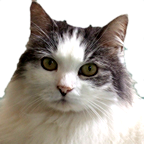
\includegraphics[width=1.5cm]{suzie.png}};
  \end{tikzpicture}
}

\title[pbkdf2]{PBKDF2: performance matters}
\author{Joseph Birr-Pixton\\
@jpixton\\
http://jbp.io/}
\date{}

\begin{document}

\frame{\titlepage}

\frame
{
  \begin{columns}[c]
    \column{.48\textwidth}
      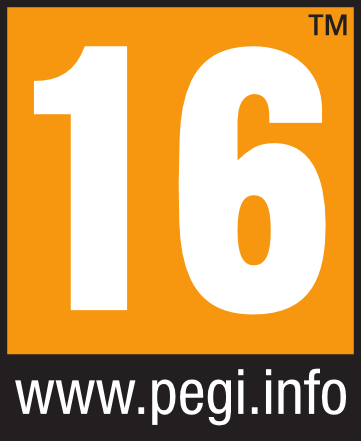
\includegraphics[width=4.7cm]{imgs/16years.png}\vspace{1mm}

      
\includegraphics[width=1.5cm]{imgs/anger.png}\hspace{1mm}
\includegraphics[width=1.5cm]{imgs/crypto.png}\hspace{1mm}
\includegraphics[width=1.5cm]{imgs/standards.png}
    \column{.48\textwidth}
      \begin{enumerate}
        \item<1> Quick intro to PBKDF2
        \item<2> The standard is bad
        \item<3> Your implementation is bad
        \item<4> A faster PBKDF2
      \end{enumerate}
  \end{columns}
}

\frame
{
  \beginner \frametitle{Intro: Merkle-Damg\r{a}rd hash functions}

  Basic construction of most hash functions: MD5, SHA-1, SHA-2.

  \begin{center}
  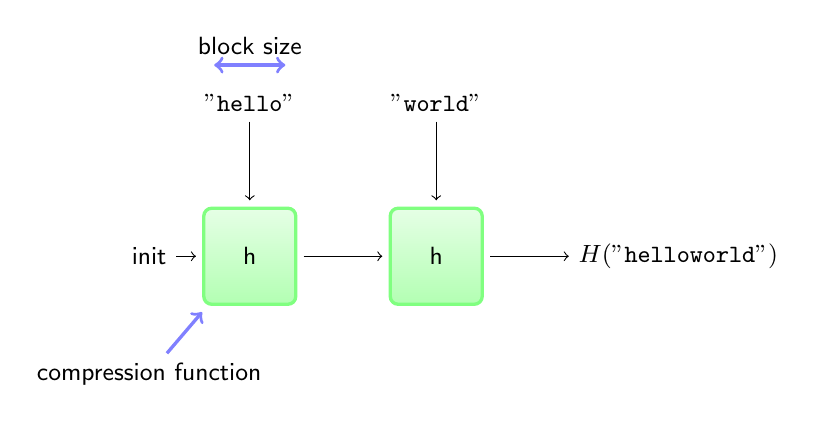
\begin{tikzpicture}[
    y = .25cm,
    x = .25cm,
    font = \small\sffamily,
    compf/.style = {
      rectangle,
      draw=green!50,
      rounded corners=1mm,
      top color=green!10,
      bottom color=green!30,
      very thick,
      inner sep=5mm,
      outer sep=1mm
    },
    labela/.style = {
      draw=blue!50,
      very thick
    }
  ]

    \node (init) {init};
    \node[compf] (h0) [right=1 of init] {h};
    \node[compf] (h1) [right=of h0] {h};
    \node (x0) [above=of h0] {$"\texttt{hello}"$};
    \node (x1) [above=of h1] {$"\texttt{world}"$};
    \node (final) [right=of h1] {$H("\texttt{helloworld}")$};
    \draw [->] (init) -- (h0);
    \draw [->] (h0) -- (h1);
    \draw [->] (h1) -- (final);
    \draw [->] (x0) -- (h0);
    \draw [->] (x1) -- (h1);

    \uncover<2>{
      \node (clabel) [below=of init] {compression function};
      \draw [->,labela] (clabel) -- (h0);

      \draw [<->,labela] ($ (x0.north west) + (1,1) $) -- ($ (x0.north east) + (-1,1) $)
        node [above,align=center,midway] {block size};
    }

  \end{tikzpicture}
  \end{center}
}

\frame
{
  \beginner \frametitle{Intro: HMAC}

  Making secure symmetric signatures out of MD hash functions.

  \begin{center}
  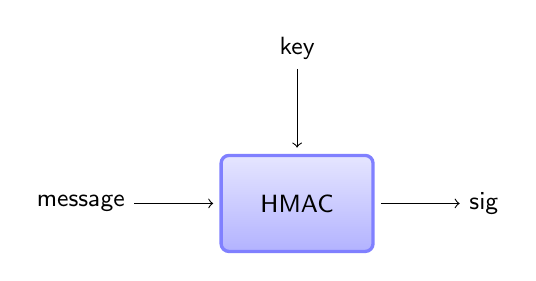
\begin{tikzpicture}[
    y = .25cm,
    x = .25cm,
    font = \small\sffamily,
    compf/.style = {
      rectangle,
      draw=green!50,
      rounded corners=1mm,
      top color=green!10,
      bottom color=green!30,
      very thick,
      inner sep=5mm,
      outer sep=1mm
    },
    hmacf/.style = {
      rectangle,
      draw=blue!50,
      rounded corners=1mm,
      top color=blue!10,
      bottom color=blue!30,
      very thick,
      inner sep=5mm,
      outer sep=1mm
    },
    labela/.style = {
      draw=blue!50,
      very thick
    }
  ]
    \node[hmacf] (expo) {HMAC};
    \node (sig) [right=of expo] {sig};
    \node (key) [above=of expo] {key};
    \node (msg) [left=of expo] {message};
    \draw[->] (expo) -- (sig);
    \draw[->] (key) -- (expo);
    \draw[->] (msg) -- (expo);
  \end{tikzpicture}
  \end{center}
}

\frame
{
  \frametitle{Intro: HMAC innards} \beginner

  \begin{center}
  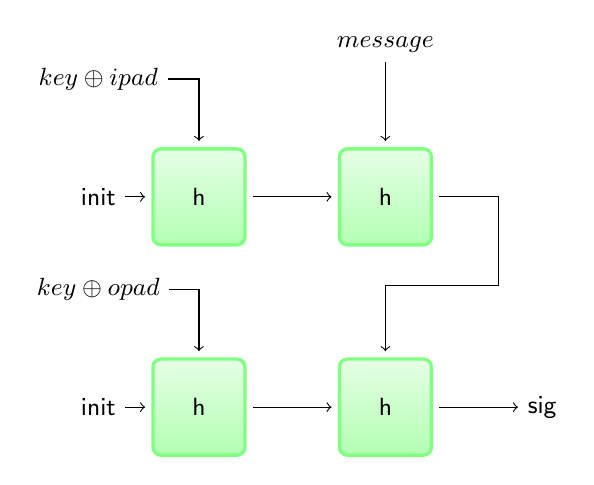
\begin{tikzpicture}[
    y = .25cm,
    x = .25cm,
    font = \small\sffamily,
    compf/.style = {
      rectangle,
      draw=green!50,
      rounded corners=1mm,
      top color=green!10,
      bottom color=green!30,
      very thick,
      inner sep=5mm,
      outer sep=1mm
    },
    hmacf/.style = {
      rectangle,
      draw=blue!50,
      rounded corners=1mm,
      top color=blue!10,
      bottom color=blue!30,
      very thick,
      inner sep=5mm,
      outer sep=1mm
    },
    labela/.style = {
      draw=blue!50,
      very thick
    }
  ]
    \node[compf] (hi0) {h};
    \node[compf] (hi1) [right=of hi0] {h};
    \node[compf] (ho0) [below=5 of hi0] {h};
    \node[compf] (ho1) [below=5 of hi1] {h};

    \draw[->] (hi0) -- (hi1);
    \draw[->] (ho0) -- (ho1);

    \node (initi) [left=1 of hi0] {init};
    \node (inito) [left=1 of ho0] {init};

    \draw[->] (initi) -- (hi0);
    \draw[->] (inito) -- (ho0);

    \node (ki) [above=of initi] {$key \oplus ipad$};
    \node (ko) [above=of inito] {$key \oplus opad$};
    \node (msg) [above=of hi1] {$message$};

    \draw[->] (ki) -| (hi0);
    \draw[->] (ko) -| (ho0);
    \draw[->] (msg) to (hi1);

    \draw[->] (hi1.east) -- ++(3,0) -- ++(0,-4.5) -| (ho1);

    \node (sig) [right=of ho1] {sig};
    \draw[->] (ho1) -- (sig);

  \end{tikzpicture}

  {\small
  $\text{HMAC-H}(key, message) \coloneqq \text{H}(key \oplus \text{opad}\ \Vert\ \text{H}({key \oplus \text{ipad}}\ \Vert\ message))$
  }

  {\footnotesize (for messages shorter than a block!) }
  \end{center}
}

\frame
{
  \beginner \frametitle{Intro: PBKDF2}

  Slowly derive a key from a password and salt.

  \begin{center}
  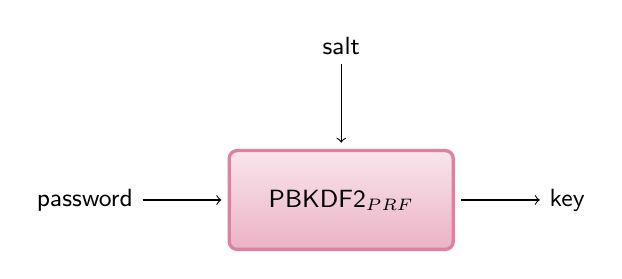
\begin{tikzpicture}[
    y = .25cm,
    x = .25cm,
    font = \small\sffamily,
    compf/.style = {
      rectangle,
      draw=green!50,
      rounded corners=1mm,
      top color=green!10,
      bottom color=green!30,
      very thick,
      inner sep=5mm,
      outer sep=1mm
    },
    hmacf/.style = {
      rectangle,
      draw=blue!50,
      rounded corners=1mm,
      top color=blue!10,
      bottom color=blue!30,
      very thick,
      inner sep=5mm,
      outer sep=1mm
    },
    kdff/.style = {
      rectangle,
      draw=purple!50,
      rounded corners=1mm,
      top color=purple!10,
      bottom color=purple!30,
      very thick,
      inner sep=5mm,
      outer sep=1mm
    },
    labela/.style = {
      draw=blue!50,
      very thick
    }
  ]
    \node[kdff] (expo) {PBKDF2$_{PRF}$};
    \node (key) [right=of expo] {key};
    \node (salt) [above=of expo] {salt};
    \node (password) [left=of expo] {password};
    \draw[->] (expo) -- (key);
    \draw[->] (password) -- (expo);
    \draw[->] (salt) -- (expo);
  \end{tikzpicture}
  \end{center}

  \begin{itemize}
    \item<2> Parameterised with a PRF, usually HMAC.
    \item<3> Tunable computation cost, with iteration count.
    \item<4> Origin: RSA labs, 1999. Described in PKCS\#5 and then RFC2898.
  \end{itemize}
}

\frame
{
  \beginner \frametitle{Intro: PBKDF2}

  \begin{block}{Iteration count choice}<1>
    \begin{enumerate}
      \item Choose computation budget (say, 50ms).
      \item Find iteration count which takes that long with your implementation.
    \end{enumerate}
  \end{block}

  \begin{alertblock}{Performance}<2>
    Performance profile is \emph{important} for defenders.  Aim: to
    maximise attacker work for defender computation budget.
  \end{alertblock}

  \begin{exampleblock}{Simplification}<3>
    PBKDF2 can produce arbitrary length output.

    We're going to ignore this capability: assume it produces
    the same length output as the underlying hash.
    %\footnote{because it's broken, and complicates matters}
  \end{exampleblock}
}

\frame
{
  \beginner \frametitle{Intro: PBKDF2$_{HMAC}$ with 3 iterations}

  \begin{center}
  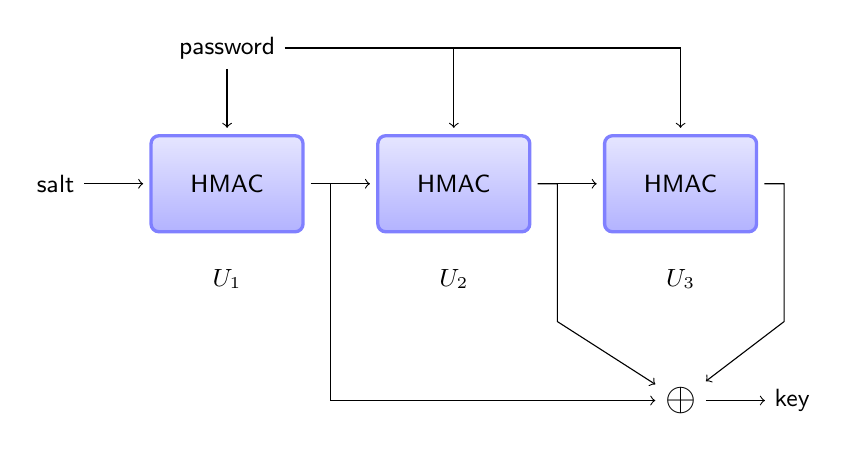
\begin{tikzpicture}[
    y = .25cm,
    x = .25cm,
    font = \small\sffamily,
    compf/.style = {
      rectangle,
      draw=green!50,
      rounded corners=1mm,
      top color=green!10,
      bottom color=green!30,
      very thick,
      inner sep=5mm,
      outer sep=1mm
    },
    hmacf/.style = {
      rectangle,
      draw=blue!50,
      rounded corners=1mm,
      top color=blue!10,
      bottom color=blue!30,
      very thick,
      inner sep=5mm,
      outer sep=1mm
    },
    kdff/.style = {
      rectangle,
      draw=purple!50,
      rounded corners=1mm,
      top color=purple!10,
      bottom color=purple!30,
      very thick,
      inner sep=5mm,
      outer sep=1mm
    },
    labela/.style = {
      draw=blue!50,
      very thick
    }
  ]
    \node[hmacf] (u1) {HMAC};
    \node[hmacf] (u2) [right=3 of u1] {HMAC};
    \node[hmacf] (u3) [right=3 of u2] {HMAC};
    \node (salt) [left=3 of u1] {salt};
    \node (password) [above=3 of u1] {password};
    \node [below=1 of u1] {$U_1$};
    \node [below=1 of u2] {$U_2$};
    \node [below=1 of u3] {$U_3$};

    \node [below=7 of u3] (gather) {\Large $\oplus$};
    \node [right=3 of gather] (key) {key};

    \draw[->] (password) -- (u1);
    \draw[->] (password) -| (u2);
    \draw[->] (password) -| (u3);
    \draw[->] (salt) -- (u1);
    \draw[->] (u1) -- (u2);
    \draw[->] (u2) -- (u3);
    \draw[->] (gather) -- (key);

    \draw[->] (u1.east) -- ++(1,0) -- ++(0,-5) |- (gather);
    \draw[->] (u2.east) -- ++(1,0) -- ++(0,-7) -- (gather);
    \draw[->] (u3.east) -- ++(1,0) -- ++(0,-7) -- (gather);

  \end{tikzpicture}
  {\footnotesize 
  \begin{align*}
    \text{PBKDF2}_\text{HMAC}(\text{password}, \text{salt}, \text{i}) &\coloneqq U_1 \oplus U_2 \oplus \cdots \oplus U_\text{i} \\
    \text{where} \\
    U_1 &\coloneqq \text{HMAC}(\text{password}, \text{salt}) \\
    U_n &\coloneqq \text{HMAC}(\text{password}, U_{n-1}) \\
  \end{align*}
  }

  \end{center}
}

\frame
{
  \beginner \frametitle{PBKDF2: perf vs. iteration count}

  One HMAC per iteration.

  \begin{center}
  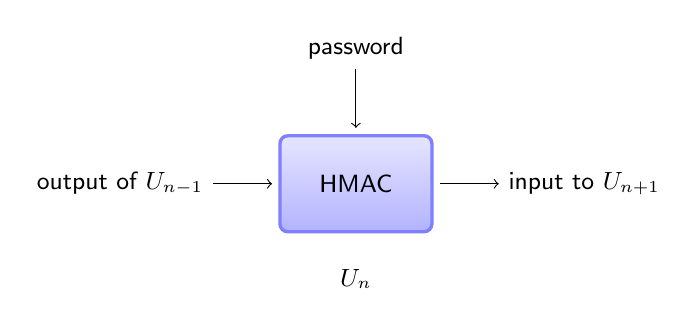
\begin{tikzpicture}[
    y = .25cm,
    x = .25cm,
    font = \small\sffamily,
    compf/.style = {
      rectangle,
      draw=green!50,
      rounded corners=1mm,
      top color=green!10,
      bottom color=green!30,
      very thick,
      inner sep=5mm,
      outer sep=1mm
    },
    hmacf/.style = {
      rectangle,
      draw=blue!50,
      rounded corners=1mm,
      top color=blue!10,
      bottom color=blue!30,
      very thick,
      inner sep=5mm,
      outer sep=1mm
    },
    kdff/.style = {
      rectangle,
      draw=purple!50,
      rounded corners=1mm,
      top color=purple!10,
      bottom color=purple!30,
      very thick,
      inner sep=5mm,
      outer sep=1mm
    },
    labela/.style = {
      draw=blue!50,
      very thick
    }
  ]
    \node[hmacf] (un) {HMAC};
    \node (inp) [left=3 of un] {output of $U_{n-1}$};
    \node (out) [right=3 of un] {input to $U_{n+1}$};
    \node (password) [above=3 of un] {password};
    \node [below=1 of un] {$U_n$};

    \draw[->] (password) -- (un);
    \draw[->] (inp) -- (un);
    \draw[->] (un) -- (out);

  \end{tikzpicture}
  \end{center}

  How many compression function applications?
}

\frame
{
  \frametitle{PBKDF2: perf vs. iteration count}

  \begin{center}
  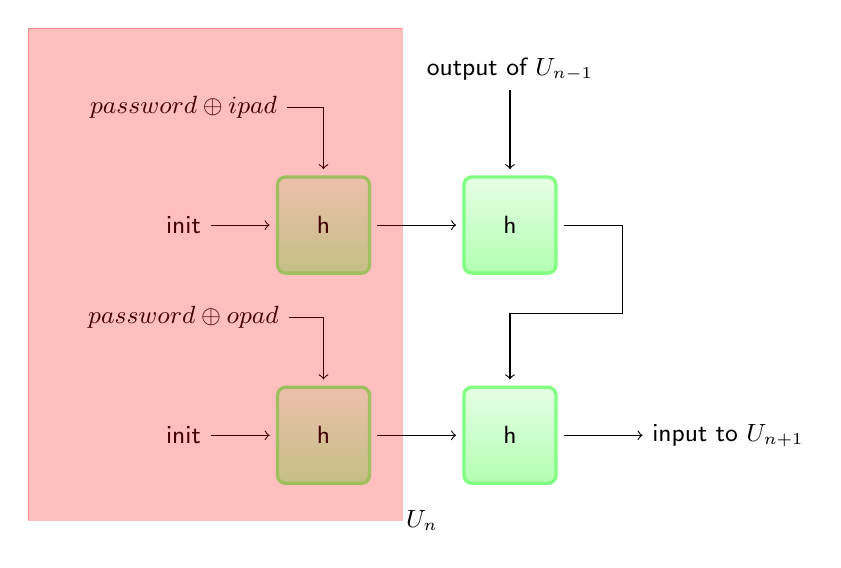
\begin{tikzpicture}[
    y = .25cm,
    x = .25cm,
    font = \small\sffamily,
    compf/.style = {
      rectangle,
      draw=green!50,
      rounded corners=1mm,
      top color=green!10,
      bottom color=green!30,
      very thick,
      inner sep=5mm,
      outer sep=1mm
    },
    hmacf/.style = {
      rectangle,
      draw=blue!50,
      rounded corners=1mm,
      top color=blue!10,
      bottom color=blue!30,
      very thick,
      inner sep=5mm,
      outer sep=1mm
    },
    labela/.style = {
      draw=blue!50,
      very thick
    }
  ]
    \node[compf] (hi0) {h};
    \node[compf] (hi1) [right=of hi0] {h};
    \node[compf] (ho0) [below=5 of hi0] {h};
    \node[compf] (ho1) [below=5 of hi1] {h};

    \draw[->] (hi0) -- (hi1);
    \draw[->] (ho0) -- (ho1);

    \node (initi) [left=3 of hi0] {init};
    \node (inito) [left=3 of ho0] {init};

    \draw[->] (initi) -- (hi0);
    \draw[->] (inito) -- (ho0);

    \node (ki) [above=of initi] {$password \oplus ipad$};
    \node (ko) [above=of inito] {$password \oplus opad$};
    \node (msg) [above=of hi1] {output of $U_{n-1}$};

    \draw[->] (ki) -| (hi0);
    \draw[->] (ko) -| (ho0);
    \draw[->] (msg) to (hi1);

    \draw[->] (hi1.east) -- ++(3,0) -- ++(0,-4.5) -| (ho1);

    \node (sig) [right=of ho1] {input to $U_{n+1}$};
    \draw[->] (ho1) -- (sig);

    \node at (5,-15) {$U_n$};

    \uncover<3>{
    \filldraw[red,nearly transparent] (-15,10) rectangle (4, -15);
    }

  \end{tikzpicture}

  \end{center}

  \alt<2->{
    \textcolor{red}{Conclusion: $4i$ compression function applications for $i$ iterations?}
  }{
    Conclusion: $4i$ compression function applications for $i$ iterations.
  }

}

\frame
{
  \frametitle{Zoom, enhance}

  The function $\text{PBKDF2}_{\text{HMAC-SHA-256}}$ is slow because it
  executes the SHA-256 compression function many times.

  \begin{block}{How many times?}<2->
    Assumption: password and salt much shorter than SHA-256's 64-byte block size.
  \begin{align*}
    \text{HMAC-H}(key, msg) &\coloneqq
      \text{H}(\alert<5>{key \oplus \text{opad}}\ \Vert\ 
      \alert<6>{\text{H}(\alert<3>{key \oplus \text{ipad}}\ \Vert\ \alert<4>{msg})}) \\
    \onslide<3>{\text{block 1} &: key \oplus \text{ipad}} \\
    \onslide<4>{\text{block 2} &: msg} \\
    \onslide<5>{\text{block 3} &: key \oplus \text{opad}} \\
    \onslide<6>{\text{block 4} &: \text{block 2 output}}
  \end{align*}

  \uncover<7->{Therefore, we need to compute $4\text{i}$ SHA-256 blocks.}
  \end{block}
}

\frame
{
  \frametitle{Nope!}

  This is suboptimal.  Neither of the standards mention this, or
  even describe the expected performance :(

  \only<1>{\vspace{1cm}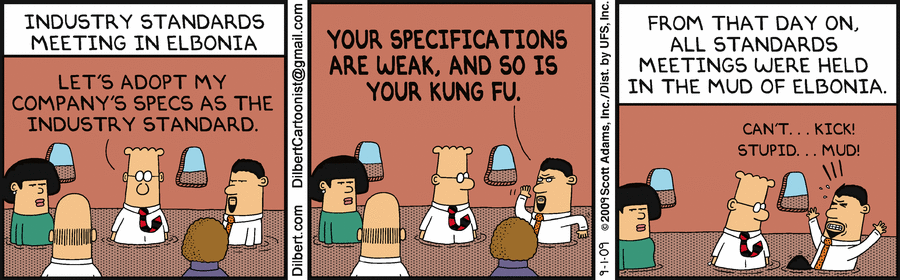
\includegraphics[width=11cm]{imgs/dilbert-2009-09-01.png}}

  \begin{align*}
    \onslide<2->{
    & U_1 \oplus U_2 \oplus \cdots \oplus U_\text{i} \\
    }
    \onslide<3->{
      \text{with} \\
      U_1 &\coloneqq \text{HMAC-H}(\text{pw}, \text{salt}) \\
      U_n &\coloneqq \text{HMAC-H}(\text{pw}, U_{n-1}) \\
    }
    \onslide<4->{
      \text{(or equivalently)} \\
      U_1 &\coloneqq \text{H}(\alert<5->{\text{pw} \oplus \text{opad}}\ \Vert\ \text{H}(\alert<5->{pw \oplus \text{ipad}}\ \Vert\ \text{salt})) \\
      U_n &\coloneqq \text{H}(\alert<5->{\text{pw} \oplus \text{opad}}\ \Vert\ \text{H}(\alert<5->{pw \oplus \text{ipad}}\ \Vert\ U_{n-1}))
    }
  \end{align*}

  \uncover<5->{We can compute these blocks once.}

  \begin{block}{How many times?}<6->
    Actually, we only need compute $2 + 2i$ SHA-256 blocks.
  \end{block}
}

\frame
{
  \frametitle{Survey of defender implementations}

  I looked at the following PBKDF2s:

  \begin{columns}[T]
    \column{.48\textwidth}
    \begin{itemize}
      \item FreeBSD 10
      \item GRUB 2.0
      \item Truecrypt 7.1a
      \item Android (disk encryption)
      \item Android (BouncyCastle)
      \item Django
      \item OpenSSL
      \item Python core ($\ge$3.4)
      \item Python (pypi pbkdf2)
      \item Ruby (pbkdf2 gem)
      \item Go (go.crypto)
    \end{itemize}
    \column{.48\textwidth}
    \begin{itemize}
      \item OpenBSD
      \item PolarSSL/mbedTLS
      \item CyaSSL/wolfSSL
      \item SJCL
      \item Java
      \item Common Lisp (ironclad)
      \item Perl (Crypt::PBKDF2)
      \item PHP5
      \item .NET framework
      \item scrypt/yescrypt\footnotemark
      \item BouncyCastle
    \end{itemize}
  \end{columns}
  
  \footnotetext[1]{never called for scrypt/yescrypt with iterations != 1}
}

\frame
{
  \frametitle{Our survey says...}

  \begin{columns}[T]
    \column{.48\textwidth}
    \begin{exampleblock}{Good: compute $2 + 2i$ blocks}
      \begin{itemize}
        \item SJCL
        \item<2-> OpenSSL (after Nov 2013)
        \item<2-> Python core ($\ge$3.4)
        \item<2-> Django (CVE-2013-1443, sc00bz)
        \item<2-> BouncyCastle ($\ge$1.49)
      \end{itemize}
    \end{exampleblock}
   
    \uncover<3->{
    \begin{alertblock}{Slow: compute $4i$ blocks}
      \begin{itemize}
        \item FreeBSD 10
        \item GRUB 2.0
        \item Android (BouncyCastle)
      \end{itemize}
    \end{alertblock}
    }

    \column{.48\textwidth}
    \uncover<4->{
    \begin{alertblock}{Slow: compute $4i$ blocks}
      \begin{itemize}
        \item Python (pypi pbkdf2)
        \item Ruby (pbkdf2 gem)
        \item Go (go.crypto)
        \item OpenBSD
        \item PolarSSL/mbedTLS
        \item CyaSSL/wolfSSL
        \item Java (OpenJDK)
        \item Common Lisp (ironclad)
        \item Perl (Crypt::PBKDF2)
        \item PHP
        \item .NET framework
        \item ...
      \end{itemize}
    \end{alertblock}
    }

  \end{columns}
}

\frame
{
  \frametitle{Selected performance measurements}

  \begin{itemize}
    \item<1> Question: how much practical difference does this make?
    \item<2> Let's measure PBKDF2-HMAC-SHA1 for large iteration count ($2^{22}$)
  \end{itemize}

  \uncover<3>{
  \vspace{2em}
  {\small Measured on Intel Atom N2800 (1.86GHz), best of five runs, CPU time in user mode.}
  }
}

\frame
{
  \frametitle{Selected performance measurements}

  \input measurements.tex

  \begin{figure}
  \centering

  \begin{tikzpicture}[
    y = .25cm,
    x = .7cm,
    font = \small\sffamily,
    fast/.style = {circle, draw=green!50, fill=green!20, thick, inner sep=0.8mm, outer sep=1mm},
    maybefast/.style = {circle, draw=green!25, fill=green!10, thick, inner sep=0.8mm, outer sep=1mm},
    slow/.style = {circle, draw=red!50, fill=red!20, thick, inner sep=0.8mm, outer sep=1mm},
    thing/.style = {font=\footnotesize},
    maybe/.style = {draw=black!50},
  ]
    \draw (0,0) -- coordinate (y axis mid) (0,22);
    \draw (0,0) -- (14,0);
    \foreach \y in {0,2,...,22} {
      \draw (0pt,\y) -- (-3pt,\y) node[anchor=east] {\y};
      \draw (0,\y) -- (14,\y) [gray!30];
    }
    \foreach \y in {1,3,...,21} {
      \draw (0pt,\y) -- (-1pt,\y);
    }
    \node[rotate=90, above=0.8cm] at (y axis mid) {Seconds};

    \node[fast,label=right:\openssltime] at (1,\openssltime) {};
    \node[thing] at (1,-1.5) {OpenSSL};

    \uncover<2-> {
    \node[fast,label=right:\pythontime] at (3,\pythontime) {};
    \node[thing] at (3,-3) {Python 3.4};
    % all openssl/openssl-derived
    }

    \uncover<3-> {
    \node[slow,label=right:\phptime] (php) at (5,\phptime) {};
    \node[thing] at (5,-1.5) {PHP5};

    \node[slow,label=right:\javaopenjdktime] (java) at (7,\javaopenjdktime) {};
    \node[thing] at (7,-3) {Java};

    \node[slow,label=right:\golangtime] (golang) at (9,\golangtime) {};
    \node[thing] at (9,-1.5) {Go};
    }

    \visible<4-5> {
    \node[fast,label=right:\phppatchtime] (phppatch) at (5,\phppatchtime) {};
    \draw [->] (php) -- (phppatch);
    % pull req https://github.com/php/php-src/pull/1387
    }

    \visible<5> {
    \node[maybefast,label=right:?] (javamaybefast) at (7,\javaopenjdktime*\phppatchtime/\phptime) {};
    \draw [maybe,->] (java) -- (javamaybefast);

    \node[maybefast,label=right:?] (golangmaybefast) at (9,\golangtime*\phppatchtime/\phptime) {};
    \draw [maybe,->] (golang) -- (golangmaybefast);
    }

    \uncover<6-> {
    \node[fast,label=right:\fastpbkdftime] at (11,\fastpbkdftime) {};
    \node[thing] at (11,-3) {fastpbkdf2};
    }

  \end{tikzpicture}
  
  \caption{PBKDF2-HMAC-SHA1, one block output, $2^{22}$ iterations}
  \end{figure}

}

\frame
{
  \frametitle{fastpbkdf2}

  A faster PBKDF2-HMAC-\{SHA-1,SHA-256,SHA-512\} for defenders.

  \begin{itemize}
    \item<1-> About 400 lines of C99.
    \item<2-> Uses OpenSSL libcrypto's hash functions.
    \item<3-> CC0.
    \item<4-> https://github.com/ctz/fastpbkdf2/
  \end{itemize}
}

\frame
{
  \frametitle{Parting thoughts...}

  \begin{itemize}
    \item<1-> PBKDF2 is a poor design, and described in an unhelpful way by its authors.
    \item<2-> Most implementations waste time and power.
    \item<3-> If you use PBKDF2, you can probably drop in a faster implementation\only<3>{.}
              \only<4>{and either
              increase security margin, or improve time/power performance.}
    \item<4-> Please try not to use PBKDF2 any more.
  \end{itemize}
}

\frame
{
  \frametitle{Thank you!}
  Questions?

  \vspace{5em}

  Twitter: @jpixton

  Mail: jbp@jbp.io

  Web: https://jbp.io/

  Slides and benchmarking code: https://github.com/ctz/talks/
}

\end{document}
